\documentclass[11pt]{article}

%%% These are some packages that are useful
\usepackage{amsmath,amssymb, amscd,amsbsy, amsthm, enumerate}
\usepackage[export]{adjustbox}
\usepackage{lastpage}
\usepackage[top=1in, bottom=1in, left=1in, right=1in]{geometry}
\usepackage[unicode]{hyperref}
\usepackage{tikz, pgfplots, xcolor, fancyhdr}
\usepackage{multicol}
\usepackage{lipsum}

%%% Page formatting
%\setlength{\headsep}{30pt}
\setlength{\textheight}{9in}
\newcommand{\tab}{\hspace{1cm}}
%\setlength{\parindent}{25pt}

\title{The Enigma of a Forgotten Prodigy}
\author{Antonius Torode}

%%% Header and Footer Info
\pagestyle{fancy}
\fancyhead[L]{{\large D\&D Character Backstory}}
\fancyhead[C]{}
\fancyhead[R]{Xavius}


\fancyhf{} % sets both header and footer to nothing
\renewcommand{\headrulewidth}{0pt}
% your new footer definitions here

\fancyfoot[L]{MSU}
\fancyfoot[C]{}
\fancyfoot[R]{\thepage\ of \pageref{LastPage}}

% Used to define spacing and format of References
\let\OLDthebibliography\thebibliography
\renewcommand\thebibliography[1]{
	\OLDthebibliography{#1}
	\setlength{\parskip}{0pt}
	\setlength{\itemsep}{0pt plus 0.3ex}
}

%%% Document Starts now
\begin{document}

\maketitle
\thispagestyle{fancy}

Battered and broken. Dizzy and shaken. As I lift myself from where I lay, my limbs shake and twitch. My vision blurred as I struggle to retain focus. Trying to pull myself up to my knees, then I collapsed. The strength within me was all but gone, and the will to move was not within me. Instead, another thought plagued my mind. Wh... what happened? I had no idea where I was or how I had gotten to the point of weakness I was in. Every bone in my body was shaking, yet I could not control them. I had the feeling of nothingness throughout my body, my energy had literally been depleted to that of nothing. As I lay there, the thought that death will overcome me seemed comforting. I let it happen, and as I lay there, I let my thoughts turn black, and enter an endless dream. 

It felt like eons that I was in that place, calm and bliss, but then... a voice. "Xavius." It was softer than an angel’s touch, lighter than the pull of space. But for some reason, it empowered me. Not physically, but in spirit. I awoke once again. Feeling worse than before, I use all my will to pull myself up from the ground. My ears were ringing. Now on my hands and knees, my vision still gone, my muscles all activated, feeling as if I had just lifted the world. My breathing was heavy, I couldn't catch my breath. The air was thin, like a fire had burned in every inch of that place. Slowly as my breathing slowed, my vision started coming back. Still blurry, it appeared as though there were lights around me. I closed my eyes and sat there for a short period of time in hopes of recovering.

Once I could catch my breath, my vision started to return. The first thing I saw was light. But it was a dim light, a glow. The ground around me, perhaps in a 5-meter diameter appeared scorched, but not with fire. The entire area was dimly glowing a light green glow. What appeared to be steam emanated from the surface. What was I doing in the center of it? Where was I? My vision returned to me slowly more and more each second, and with it my ears rang less and less. It appeared as though I was in a dark cavern. Beyond the area that was glowing, was rocky terrain, with what appeared as corpses. They were not ordinary corpses though, not that of dwarves or humans, or elves or gnomes. These corpses appeared to be that of void, dark creatures. A purple haze emanated from the remains. The feeling of raw power was surrounding me in the air.

Despite all this, I had no idea what had brought me there, how I got there, or even who I was. It was as if my memory had been wiped. I still knew the languages I was brought up with but couldn't remember my parents. I still knew what my hands and feet were but couldn't recall any memories of me using them. It was the strangest feeling ever. To feel like you've done things a million times but never recall doing anything. 

There on the ground were a few objects. One of which was a staff which turned to ash in my hands. Another object was a book. The book had a single word on the cover, an ambigram of the word "Xavius."

\begin{center}
	
\includegraphics[]{./ambigram.png}
\end{center}

I picked up the book and opened it. The entire thing was written in writings that were foreign to me. However, the strange part is that it was my handwriting. I knew this immediately after seeing it even though I had no idea what was written. This raised yet another question, how could I recognize my handwriting but not even know who I was. It did not mean much to me at the time, because I still had no energy and no idea where I was or how I was going to escape.

Among the other items there was a small vial. I had no idea what the contents were, but there was a thin red liquid inside. Knowing I was doomed in my current state, I took the risk. It was a bit of a struggle, but the thin liquid went smoothly down my throat. As it did, a tingling feeling, perhaps burning as it went down. I had never felt anything quite like it since. Regardless, my vitality had immediate improvement, and within about 15 minutes or so, miraculously restored. 

It was very un-easy being in that place. I gathered what I could and searched for an exit. It must have been a whole day or two before finding me way out. It's a miracle I even did. There was no light once I left that initial area and the terrain was very dangerous. Unfortunately, upon exiting that cave I was in, I was now on the side of a large cliff overlooking a large forest. I would have thought I had been hungry by then but whatever was in that vial was sustaining me for the time being. I rested a while at the mouth of that cave, but quickly took back up and headed out.

While resting there I only came upon more questions. The book was a complete mystery, but I knew that if I could decipher it then perhaps it could explain more about my past. Among the other items there did not appear to be anything significant. Little trinkets, a bag of dust, a small rod, 3 silver coins, etc. I headed out shortly after that. I wondered for days until I came across a pasture where I was able to trade some of my trinkets for supplies. The Sheppard there pointed me in the direction of a nearby city. For some reason he had made a big deal about how he had never seen such a strong half-elf. Regardless, I have since lost my physique by the struggles to survive and dedication to study. On both of my forearms were golden diamonds embedded into my skin. Within the diamonds were gems. On the right hand, a white gem, and on the left, a black. I later found out from a jewel crafter that this was a very old technique where the skin was carved, and wounds filled and cauterized with molten metal. It's supposedly a form of art.

It has been 2 years since then. I've been traveling in the hopes of discovering more about the book. From what I've gathered, it is no known language. Apart from that, it may even be in code. Anyways this is just what the few 'language experts' I have found said. I even came across a divination master once whom can read any language and even he was at a loss. This journey so far has been mainly self-discovery. As I still do not know who I am, I did quickly learn I have a quick ability to learn. Aside from that, I appear to have an act for spell-handling.

During my travels, I came across a man named Abasi from a small city of Ramkahen. This man was a very old elf wizard. He told me this book was a spell-book. After telling him my story, he agreed and started teaching me the ways of a wizard. In hopes of understanding my past, this is what I have been doing since. Abasi died a few months later but I learned a great deal from him. After this point, I headed to a larger city where I have been studying. I joined a school of magic at first, where I started at a far disadvantage, however, it turns out I have a gifted ability to learn and quickly caught up to some who have been studying for years. As such with my past, I joined a school of Divination.

Since this time, I have been studying and searching for answers, which is what has led me to Cos. A legend of a great Wizard, Kalec. He is said to be a master of Divination, though he disappeared many years ago. I am here in Cos searching for clues on his whereabouts.



\begin{center}
	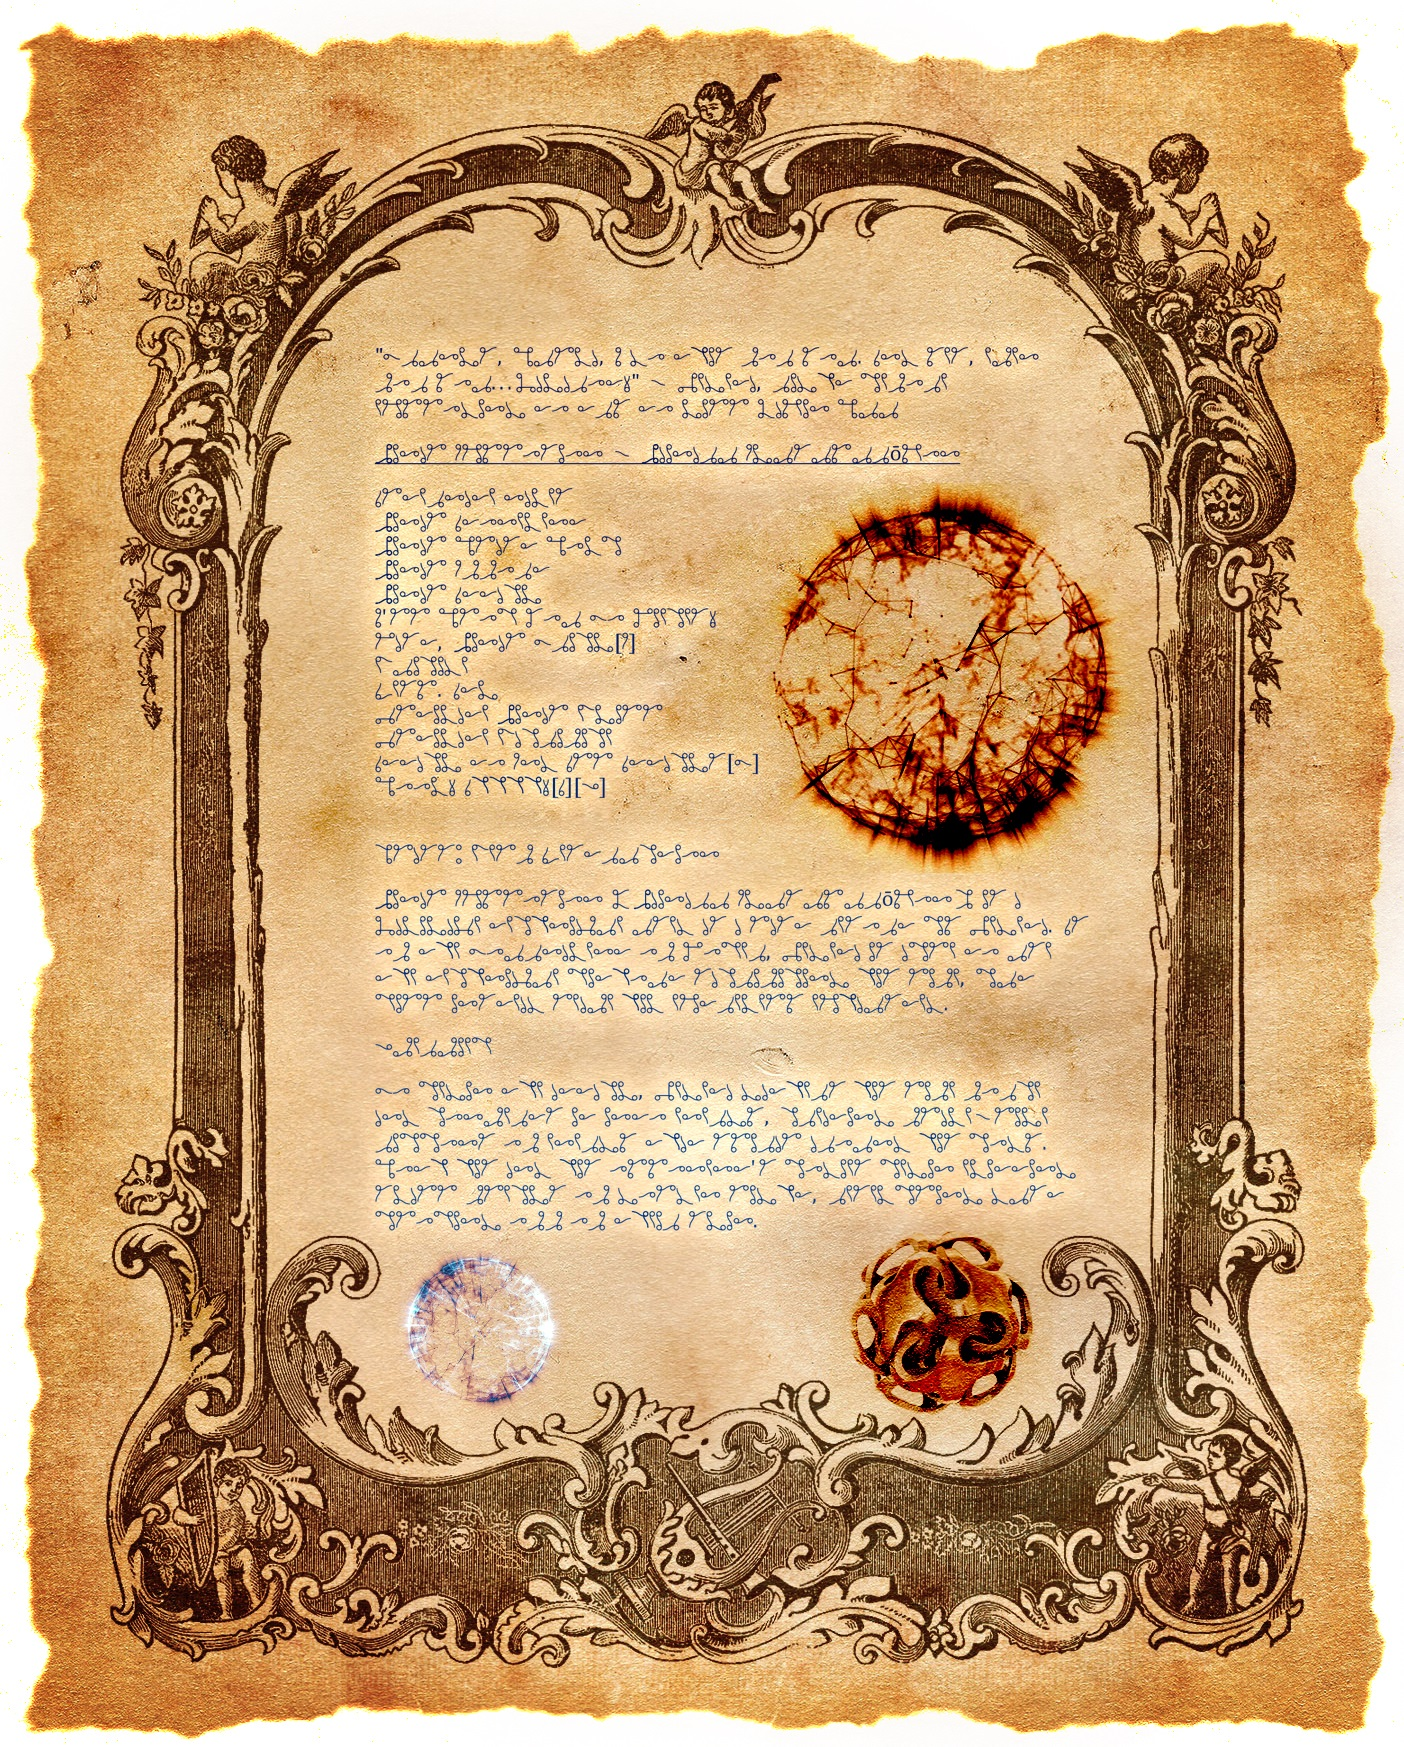
\includegraphics[]{./page.jpg}
	
	{\footnotesize A sample page from the book}
\end{center}
%%%%%%%%%%%%%%%%%%%%%%%%%%%%%%%%%%%%%%%%%%%%%%%%%%%%%%%%%%%%%%%%%%%%%%%%%%%%%%%%%%%%%%%%%%%
\end{document}





















